\chapter{Introduction}
\label{chap:context}

In this dissertation I present SFL-explorer: a tool to demonstrate how functional programming languages are evaluated, allowing users to gain a valuable intuition of these languages. 

SFL-explorer takes the form of a functional language (\ac{SFL}), packaged with two interfaces that allows users to observe the process of evaluation of a term as a series of step by step or multi-step reductions, and control the order that sub-terms are evaluated. These interfaces are a \ac{CLI} and a web application. The ultimate goal of this project was to make a tool that makes learning and teaching the basics of functional programming easier. There are two groups of people the project is designed to be of interest to:
\begin{itemize}
    \item Those involved in learning functional languages. These could be students of a university course, or anyone interested in the topic. 
    \item Those involved in teaching functional languages, as part of a university course or otherwise.
\end{itemize}

The language itself is not meant to be the main interest for the users of this system. It is designed to be fairly generic, with syntax and semantics similar to popular functional languages, so that users can take their understanding from using SFL-explorer and apply it to these languages. 

\section{COMS10016: Imperative and Functional Programming at the University of Bristol}
\label{COMS10016}
In the first year of most computer science programs at the University of Bristol, students take the module \href{https://www.bristol.ac.uk/unit-programme-catalogue/UnitDetails.jsa?unitCode=COMS10016}{COMS10016}, a combined imperative and functional programming module. This is many students first encounter with both of these types of programming. In the functional part of this unit, students are taught Haskell. The unit material is presented to students through a very effective lecture series, supplemented by weekly worksheets that students have the opportunity to work through in labs attended by the lecturers, as well as some teaching assistants. Two of the lecturers in this unit are Jess Foster and Samantha Frohlich. 

\begin{quote}
`The aim [of the functional portion of the unit] is to introduce types and functions. Important principles include datatypes, evaluation order, higher-order functions, and purity' \cite{COMS10016}
\end{quote}

\noindent I acted as a teaching assistant in the labs for two academic years. My role was to answer students questions about functional languages or the worksheets they were given. The inspiration for this project came from my experience struggling to explain key functional programming concepts, as I had no tool.

\section{Agile Development Lifecycle}
The project followed a development lifecycle inspired by Agile principles\cite{agilemanifesto2001}, structured into four iterative cycles. Each cycle built upon the last, integrating evaluation and feedback to continuously and rapidly refine the features and the UI/UX of the system. 

Each cycle was further subdivided into four phases:

\begin{itemize}
    \item \textbf{Requirements Gathering}
    \item \textbf{Design and Research}
    \item \textbf{Implementation}
    \item \textbf{Evaluation}
\end{itemize}

\begin{figure}[t]
    \centering
    \fbox{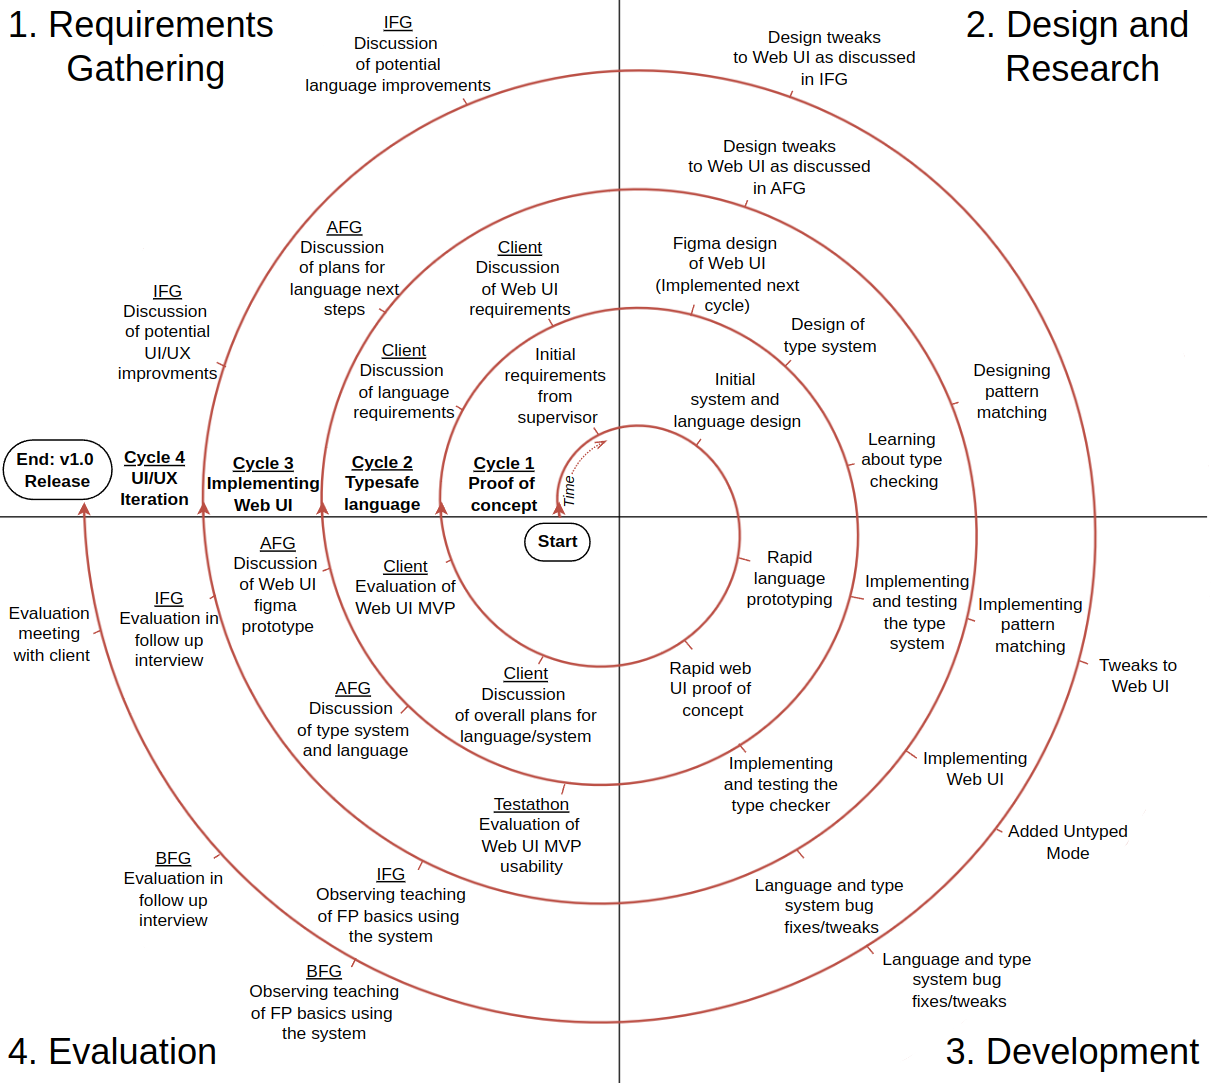
\includegraphics[width=0.98\linewidth]{images/spiral1.drawio.png}}
    \caption{A spiral representation of the project lifecycle, showing the 4 iterations, and the work done in each part of each cycle. }\label{fig:spiral}
\end{figure}

This iterative methodology helped manage complexity and uncertainty. Getting frequent feedback from users and my client allowed me to keep 


